
%
%  $Description: Author guidelines and sample document in LaTeX 2.09$ 
%
%  $Author: ienne $
%  $Date: 1995/09/15 15:20:59 $
%  $Revision: 1.4 $
%

\documentclass[times, 10pt,twocolumn]{article} 
\usepackage{latex8}
\usepackage{times}
\usepackage[ngerman]{babel}
\usepackage[utf8]{inputenc}
\usepackage{color}
\usepackage{graphicx}
\usepackage{capt-of}
\usepackage{amsmath}



%\documentstyle[times,art10,twocolumn,latex8]{article}

%------------------------------------------------------------------------- 
% take the % away on next line to produce the final camera-ready version 
\pagenumbering{arabic}

%------------------------------------------------------------------------- 
\begin{document}

\title{Distributed Computation of Disparity Maps on multiple GPUs using TCP sockets}

\author{Eric Buschermöhle, Sven Frank, Timo Janssen\\
Technische Universität Braunschweig \\  38106 Braunschweig, Deutschland\\
e.buschermoehle@tu-bs.de\\
}


\maketitle
\thispagestyle{empty}

\begin{abstract}
   The ABSTRACT is to be in fully-justified italicized text, at the top 
   of the left-hand column, below the author and affiliation 
   information. Use the word ``Abstract'' as the title, in 12-point 
   Times, boldface type, centered relative to the column, initially 
   capitalized. The abstract is to be in 10-point, single-spaced type. 
   The abstract may be up to 3 inches (7.62 cm) long. Leave two blank 
   lines after the Abstract, then begin the main text. 
\end{abstract}



%------------------------------------------------------------------------- 
\Section{Einführung}

Zum Auffinden von korrespondierenden Punkten in einem Stereobildpaar werden verschiedene Stereoanalyseverfahren eingesetzt. Mit Hilfe der gefunden Korrespondenzen und den intrinsischen sowie extrinsischen Parameter des Stereokamerasystems ist es möglich mit Triangulation eine Szene 3D rekonstruieren. Stereoanalyseverfahren finden Einsatz im Industriellen Umfeld z.B. im Bereich der Qualitätssicherung. Aber auch Anwendungsfelder in der Robotik und Automobilindustrie z.B. zur Hinderniserkennung  sind potentielle Anwendungsbereiche. Neben einer möglichst dichten und genauen Tiefenkarte spielen Laufzeitaspekte eine entscheidende Rolle. In dieser Arbeit wird das Laufzeitverhalten anhand einer Korrelationsmethode exemplarisch untersucht. Es werden insgesamt zwei Möglichkeiten zur Beschleunigung des Verfahrens vorgestellt. In einem ersten Schritt erfolgt die Parallelisierung auf der GPU (Graphics Processing Unit) mit der von Nvidia entwickelten Programmier-Technik CUDA. In einem zweiten Schritt erfolgt die Verteilung der Anwendung auf über TCP verbundene Clients. Zu diesem Zweck werden einfache TCP-Sockets eingesetzt. {\color{red}{Quelle}}

%------------------------------------------------------------------------- 
\SubSection{Korrelationsmethode}

Der Algorithmus benötigt ein Referenzbild sowie ein Suchbild, welche beide entzerrt und rektiziert sein müssen. Die Vorgehensweise zur Bestimmung der Disparität ist dabei wie folgt: Ausgehend von einem Bildpunkt $(u_1,v_1)$ im Referenzbild wird ein Referenzfenster der Größe \textit{MaskWidth} und \textit{MaskHeight} um den Aufpunkt gewählt und mit entsprechenden verschobenen Suchfenstern aus dem Suchbild entlang einer korrespondierenden Zeile (Epipolarlinie) verglichen. Dies entspricht also der Bestimmung der Ähnlichkeit zweier gleichgroßer Fenster. Unter Verwendung einer Kostenfunktion kann die Bildposition (u2; v2) ermittelt werden, die für das gewählte Referenzfenster im Referenzbild das ähnlichste Suchfenster im Suchbild darstellt d.h. die niedrigsten Kosten besitzt. Die Differenz der Punkte $(u_1,v_1)$ und $(u_2,v_2)$ wird Disparität $d(u_1,v_1)$ genannt und wird zur Bestimmung der Tiefe einer Szene benötigt. Weiterführende Literatur ist in: \cite{Hartley.2003} und \cite{Schreer.2005} zu finden. Wurden für alle Bildpunkte in einem Bild die Disparitäten gefunden, werden diese zu einer sogenannten Disparitätskarte oder auch Tiefenkarte zusammengefügt. In Abbildung \ref{fig:korrelationsmethoden} ist ein Referenzfenster und ein um die Disparität $d(u,v)$ verschobenes Suchfenster dargestellt.

\begin{figure}[!ht]
	\centering
	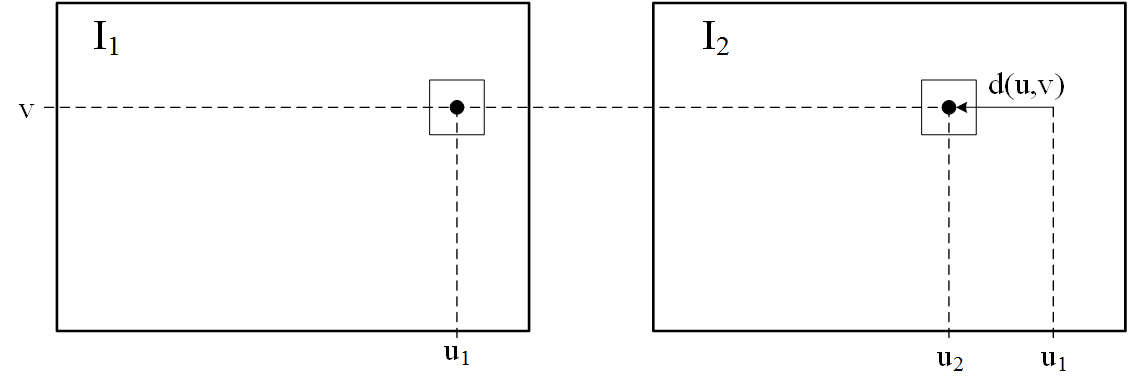
\includegraphics[width=0.9\linewidth]{image/korrelationsverfahren.png}
	\captionof{figure}[Korrelationsmethoden]{Darstellung der Fenster in beiden Bildern zur Bestimmung der Ähnlichkeit}
	\label{fig:korrelationsmethoden}
\end{figure}

%------------------------------------------------------------------------- 
\SubSection{Kostenfunktion}

Als Kostenfunktion wird in dieser Arbeit der Mittlere absoluter Fehler (engl. sum of absolute dierences (SAD)) eingesetzt. Mit diesem wird die absolute Differenz zwischen zwei Fenstern berechnet. Die Ähnlichkeit ist dort am größten, wo die Differenz minimal wird

\begin{align}
\small 
\begin{split}
C(u,v,d) = \frac{1}{N}\sum\limits_{m} \sum\limits_{n} | g_1(u+m,v+n) - \\ g_2(u+d(u,v)+m,v+n)|
\label{eq:sad}
\end{split}
\end{align}

%------------------------------------------------------------------------- 
\SubSection{Graphics Processing Unit}
Der Grafikprozessor ist eine auf Berechnung von Grafiken spezialisierter und optimierter Prozessor in einem Computer oder einem anderen Gerät mit visueller Ausgabe.
Der Cache-Speicher der GPU (Graphic Processing Unit) ist im Gegensatz der CPU erheblich kleiner dimensioniert. Zudem existiert kein Raum für komplexe Logik. Grundsätzlich ist die Recheneinheit der Grafikkarte so aufgebaut, dass möglichst viele eher einfach Rechenoperationen parallel möglich sind.
Diese Algorithmic Logic Units (ALU) sind wie in Abbildung <<NR>> dargestellt in wesentlich höhrerer Anzahl auf der GPU vorhanden. Sie lassen sich wiederum jeweils in eine bestimmte Anzahl an Blöcke unterteilen, wobei jeder Block selbst mehrere Threads aufrufen kann. Durch diese Unterteilung ermöglicht der Grafikprozessor eine wesentlich schnellere Berechnung von einfachen arithmetischen Aufgaben.

%------------------------------------------------------------------------- 
\Section{Related Work}

Die Berechnung von Tiefenkarten auf der GPU ist nicht neu. In der Arbeit von \cite{Yang.2002} wird eine Methode vorgestellt, die Korrelationsmethoden basierend auf der Kostenfunktion SAD mit Hilfe der GPU berechnet. In \cite{Woetzel.2004} erfolgt die Berechnung der Tiefenkarte mit der Kostenfunktion SSD. Die Bildvorverarbeitung und Nachbereitung erfolgt dabei ebenfalls auf der GPU. Als Ergebnis konnte eine Beschleunigung der Verarbeitungsgeschwindigkeit auf 20fps erreicht werden.

Aktuellere Arbeiten beschäftigen sich mit der Beschleunigung des von Hirschmüllers vorgestellten Semi-Global Matching (SGM) \cite{Hirschmuller.2005} zum Erzeugen von Tiefenkarten. Ein Beispiel dafür ist die Arbeit \cite{Hirschmueller.2008} und \cite{Rosenberg.2006}, in welcher die Berechnung von Tiefenkarten mit dem SGM und CUDA implementiert wurde.

{\color{red}KONNTE LEIDER KEINE LITERATUR ZU VERTEILTEN STEREOALGORITHMEN FINDEN! VIELLEICHT HABT IHR MEHR GLÜCK!
Die Verteilung von Stereoalgorithmen wird vor allem in der}

%------------------------------------------------------------------------- 
\Section{Ansatz}

In dieser Arbeit geht es zunächst daraum die Berechnung der Tiefenkarte von der CPU auf die GPU auszulagern. Dazu soll eine entsprechende Programmiertechnik verwendet werden, um die notwendigen auf den Grafikspeicher zu transferieren. Im zweiten Schritt soll die Berechnung möglichst gut optimiert werden. Hierbei soll die Rechenzeit durch weitere Parallelisierung reduziert werden.
Als letzte Möglichkeit zur Reduzierung der Zeit, soll eine Client-Sever Anwendung entwickelt werden. Dadurch soll die Berechnung auf mehrere Grafikkarten auf verschiedenen Rechnern über das Netzwerk aufgeteilt werden. Dafür soll das Bild in einzelne Segmente unterteilt werden und über das Netzwerk zur Berechnung an die verschiedenen Computer gesendet werden. Im Anschluss werden die einzelnen berechneten Segmente der Tiefenkarte zu einer gesamten Tiefenkarte zusammengefügt.

%------------------------------------------------------------------------- 
\Section{Implementierung}
\SubSection{Optimierung von CPU auf GPU}
\textbf{CUDA}

Die Programmiertechnik CUDA (Compute Unified Device Architecture) ist eine vom Grafikkarten-Hersteller nVidia entwickelte Möglichkeit, wodurch der Anwender Berechnungen auf dem Grafikprozessor ausführen kann. 
In der Kurzfassung schreibt der Entwickler einen sogenannten Kernel, welche die Rechenlogik enthält die auf der GPU ausgeführt werden soll. Zudem muss der Host-Code geschrieben werden, welcher der das eigentliche Programm in der jeweiligen Programmiersprache enthält, die notwendigen Daten über spezifische Funktionen auf die GPU transferiert und dann den Kernel aufruft. Anschließend müssten die berechneten Daten wieder von der GPU auf die CPU kopiert und dort ausgewertet werden.
Eine Parallelisierung ist hierbei durch den Entwickler möglich. Dieser kann steuern, auf wie viele Blöcke und Threads die entsprechende Operation aufgeteilt werden soll.

\SubSection{Entwicklung und Paralellisierung des Kernels}
TODO: Beschreibung des Kernels und die Parallelisierung

\SubSection{Parallelisierung über TCP/IP}

\textbf{Netzwerkkommunikation}

Bei Sockets handelt es sich um ein vom Betriebssytem bereitgestelltes Objekt, welche als Kommunikationsendpunkte betrachtet werden können. Durch diese Socktes können Daten empfangen und versendet werden, wobei verschiedene Techniken zur Übermittlung auf der Transportschicht verwendet werden können.
Ein bekanntes und im Zuge dieser Arbeit verwendetes Modell nutzt TCP/IP zur Kommunikation. Dabei sorgt das Transmission Control Protocol für eine zuverlässige Übertragung der Daten auf Basis vom Internet Protocol (IP). Die Übermittlung der Pakete ist dabei garantiert. Sollte ein Fehler auftreten, so erhält der Sender eine Fehlermeldung und kann die Daten erneut senden. Grundsätzlich entspricht die Reihenfolge der eingehenden Pakete der Sendereihenfolge.
Die Verbindung zwischen zwei Kommunikationspartnern wird bei diesem Mechanismus durch die IP-Adressen und eine gemeinsame Portnummer hergestellt.

\textbf{Client-Server Anwendung}

TODO: Beschreibung der Implementierung

%------------------------------------------------------------------------- 
\Section{Evaluation}

Ziel dieser Arbeit war es die Reduzierung der Berechnungsgeschwindigkeit zu messen, wenn die Berechung via Transmission Control Protocol (TCP)/Internet Protocol (IP) auf mehrere Grafikprozessoren auf verschiedenen Rechnern aufgeteilt wird.
Die Ausgangssoftware behinhaltete bereits die Berechung der Tiefenkarte auf der CPU, welche nicht wirklich für diese Aufgabe optimiert ist. Im ersten Schritt wurde die Anwendung also dahingehend erweitert, dass mittels der Programmier-Technik CUDA die Berechung auf der Grafikkarte (GPU) ausgeführt werden konnte.
Der zweite Schritt beinhaltete die Entwicklung einer simplen Client-Server-Anwendung. Dabei sollte der serverseitige Part die Berechung auf der GPU anstoßen. Die notwendigen Vorbereitungen auf der Clientseite, waren zum größten Teil schon in der bereitgestellten Software vorhanden. So musste sich weder um die gesamte Integration, die Aufteilung des Bildes für die entsprechende Serveranzahl, noch das spätere Zusammenfügen der Ergebnisbilder gekümmert werden. Lediglich der Kommunikationskanal musste aufgesetzt werden und die Bereitstellung der notwendingen Informationen für die Berechnung implementiert werden.

Im Zuge der Durchführung des Versuches wurde versucht die Berechungszeit der Tiefenkarte immer weiter zu reduzieren. Begonnen wurde mit der CPU, gefolgt von der GPU auf dem Host-Rechner. Anschließend wurde die Berechnung über das Netzwerk auf eine steigende Anzahl von Rechnern verteilt. 

Für den Versuch wurden immer die gleichen Parameter zur Berechnung verwendet, damit die Ergebnisse vergleichbar sind. Als Versuchsbild diente ein Bild von einem Elefanten mit einer Auflösung von 681x681 Pixel. Dabei wurde das linke und das rechte Bild bereitgestellt. Die Parameter wurden anschließend wie folgt festgelegt:

Fenstergröße: 7x7 Pixel
Taumax: 40

Die Durchführung des Versuches ergab die in Tabelle 1 dargestellten Ergebnisse.

\textbf{TABELLE}

Die Tabelle <<NR>> zeigt deutlich, dass die GPU wesentlich besser geeignet ist, um Grafikoperationen zu erledigen. Die Zeit für die Berechung der Tiefenkarte konnte auf der GPU im Vergleich zu CPU um etwas 85\% des Ausgangswertes reduziert werden. Teilt man diese Berechung nun auf mehrere GPUs über das Netzwerk auf, so stellt man fest, dass bis zu einer Verwendung von 6 GPUs die Rechenzeit noch erheblich sinkt. In fügt man nun weitere GPUs hinzu, so konvergiert die Rechenzeit irgendwann gegen einen bestimmten Wert. Bereits bei einer Erhöhung von 7 auf 8 GPUs erkennt man schon kaum eine wirkliche Reduzierung.

%------------------------------------------------------------------------- 
\Section{Zusammenfassung}

%------------------------------------------------------------------------- 
\Section{Ausblick}




%------------------------------------------------------------------------- 
\SubSection{Beispiel Footnotes}

Please use footnotes sparingly%
\footnote
   {%
     Or, better still, try to avoid footnotes altogether.  To help your 
     readers, avoid using footnotes altogether and include necessary 
     peripheral observations in the text (within parentheses, if you 
     prefer, as in this sentence).
   }
and place them at the bottom of the column on the page on which they are 
referenced. Use Times 8-point type, single-spaced.

\bibliographystyle{latex8}
\bibliography{latex8}

\end{document}

